\paragraph{QuizziPedia::Front-End::Controllers::NewQuestionsButtonController}
\begin{figure} [ht]
	\centering
	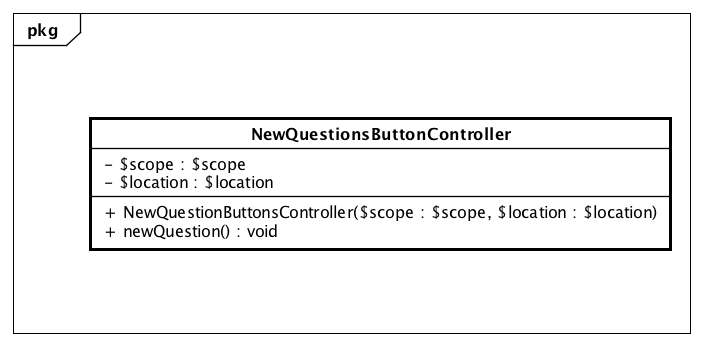
\includegraphics[scale=0.45]{UML/Classi/Front-End/QuizziPedia_Front-end_Controller_NewQuestionsButtonController.png}
	\caption{QuizziPedia::Front-End::Controllers::NewQuestionButtonController}
\end{figure} \FloatBarrier
\begin{itemize}
	\item \textbf{Descrizione}: questa classe permette di effettuare il redirect alla pagina di creazione nuova domanda;
	\item \textbf{Utilizzo}: effettua il redirect alla pagina di creazione di una nuova domanda quando l'utente seleziona interagisce con il bottone a cui è collegato il corrispettivo evento;
	\item \textbf{Relazione con altre classi}:
	\begin{itemize}
		\item \texttt{OUT} \texttt{NewQuestionsButtonDirective}: rappresenta il componente grafico che permette all'utente di posizionarsi nella view di creazione di una nuova domanda;
	\end{itemize}
	\item \textbf{Attributi}:
	\begin{itemize}
		\item \texttt{-} \texttt{\$scope: \$scope} \\
		Campo dati contenente un riferimento all’oggetto \$scope creato da \textit{Angular\ped{G}}, viene utilizzato come mezzo di comunicazione tra il controller e la view. Contiene gli oggetti che definiscono il model dell’applicazione;
		\item \texttt{-} \texttt{\$location: \$location} \\
		Campo dati contenente un riferimento al servizio creato da \textit{Angular\ped{G}} che permette di accedere alla barra degli indirizzi del \textit{browser\ped{G}}, i cambiamenti all’URL nella barra degli indirizzi si riflettono in questo oggetto e viceversa.
	\end{itemize}
	\item \textbf{Metodi}:
	\begin{itemize}
		\item \texttt{+} \texttt{NewQuestionButtonsController(\$scope: \$scope, \$location: \$location)} \\ 
		Metodo costruttore della classe. \\
		\textbf{Parametri}:
		\begin{itemize}
			\item \texttt{\$scope: \$scope} \\
			Parametro contenente un riferimento all’oggetto \$scope creato da \textit{Angular\ped{G}}. Viene utilizzato come mezzo di comunicazione tra il controller e la view. Contiene gli oggetti che definiscono il viewmodel e il model dell’applicazione;
			\item \texttt{\$location: \$location} \\
			Parametro contenente un riferimento al servizio creato da \textit{Angular\ped{G}} che permette di accedere alla barra degli indirizzi del \textit{browser\ped{G}}, i cambiamenti all’URL nella barra degli indirizzi si riflettono in questo oggetto e viceversa.
		\end{itemize}
		\item \texttt{+} \texttt{newQuestion(): Void} \\ 
		Metodo che gestisce l’evento click sul pulsante per creare una nuova domanda. Effettua il redirect alla pagina di creazione di una domanda.
	\end{itemize}
	
\end{itemize}

